% =====================================================================
%  Checkpoint 01 Report - Web E-commerce Project
%  Compile with pdfLaTeX (Overleaf default). Rename the output PDF to
%  Checkpoint_01_Report_<TeamName>.pdf before submitting.
%  Edit the values in the "TEAM INFO" block below first.
% =====================================================================
\documentclass[12pt,a4paper]{article}   % font size 12

% --- Font: set Compiler = XeLaTeX on Overleaf (Menu > Compiler) ---
\usepackage{iftex}
\ifPDFTeX
  % pdfLaTeX fallback: Vietnamese names render, but no Times New Roman
  \usepackage[T5]{fontenc}
  \usepackage[utf8]{inputenc}
\else
  % XeLaTeX/LuaLaTeX: Times New Roman, or TeX Gyre Termes (a Times clone) if missing
  \usepackage{fontspec}
  \IfFontExistsTF{Times New Roman}
    {\setmainfont{Times New Roman}}
    {\setmainfont{TeX Gyre Termes}}
\fi
\usepackage[a4paper,margin=2.2cm]{geometry}
\usepackage{amssymb}
% --- Table packages ---
\usepackage{array}             % column formatting: >{...}, p{}, m{}, b{}
\usepackage{tabularx}          % tables that stretch to the page width (X columns)
\usepackage{booktabs}          % clean rules: \toprule \midrule \bottomrule \cmidrule
\usepackage{longtable}         % long tables that break across pages
\usepackage{ltablex}           % tabularx + longtable (X columns in multi-page tables)
\keepXColumns                  % keep X column widths as in tabularx
\usepackage{multirow}          % merge rows: \multirow{2}{*}{...}
\usepackage{makecell}          % line breaks inside a cell: \makecell{line 1\\line 2}
\usepackage[table]{xcolor}     % row/cell colors: \rowcolor, \cellcolor, \rowcolors
\usepackage{caption}           % table/figure captions: \caption{...}
\usepackage{float}             % place tables exactly here: \begin{table}[H]
\usepackage{enumitem}
\usepackage{tikz}
\usetikzlibrary{positioning,arrows.meta,shapes.geometric,fit}
\usepackage{hyperref}
\hypersetup{colorlinks=true,linkcolor=blue!50!black,urlcolor=blue!60!black}

\setlist{nosep,leftmargin=1.4em}
\setlength{\parskip}{0.4em}
\setlength{\parindent}{0pt}
\renewcommand{\arraystretch}{1.25}
\newcolumntype{Y}{>{\raggedright\arraybackslash}X}               % stretchable, left-aligned
\newcolumntype{L}[1]{>{\raggedright\arraybackslash}p{#1}}        % fixed width, left-aligned
\newcolumntype{C}[1]{>{\centering\arraybackslash}p{#1}}          % fixed width, centered
\newcolumntype{M}[1]{>{\raggedright\arraybackslash}m{#1}}        % fixed width, vertically centered

\newcommand{\yes}{$\checkmark$}
\newcommand{\no}{$\times$}
\newcommand{\half}{$\circ$}

% ------------------------- TEAM INFO (EDIT) --------------------------
\newcommand{\TeamName}{WEB\_2627302\_10}
\newcommand{\ProjectName}{VoltCart}
\newcommand{\RepoURL}{\url{https://github.com/NguyenCongThanh-star/VoltCart}}
\newcommand{\MemberA}{Nguyễn Công Thành\newline (ID: ........)}
\newcommand{\MemberB}{Nguyễn Minh Mẫn\newline (ID: ........)}
\newcommand{\MemberC}{Lương Nhất Khôi\newline (ID: ........)}
\newcommand{\MemberD}{Huỳnh Nhật Hòa\newline (ID: ........)}
% ---------------------------------------------------------------------

\begin{document}

% ============================== TITLE ===============================
\begin{center}
  {\Large\bfseries Checkpoint 01 -- Team Formation and Initial Research}\\[0.4em]
  {\large Web E-commerce Project: \textbf{\ProjectName} -- Smartphones \& Laptops Store}\\[0.3em]
  Team: \textbf{\TeamName} \quad|\quad Repository: \RepoURL
\end{center}
\vspace{-0.5em}
\noindent\rule{\linewidth}{0.4pt}

% =====================================================================
\part*{\large Part A -- Project Direction}
% =====================================================================

\section{Project Overview}

\begin{tabularx}{\linewidth}{|l|Y|}
\hline
\textbf{Project name}     & \ProjectName \\ \hline
\textbf{Product category} & New consumer electronics: \emph{smartphones}, \emph{laptops},
                            and a small set of \emph{accessories} (chargers, earphones, cases). \\ \hline
\textbf{Target customers} & Students and young professionals (18--35) in Vietnam who buy a
                            phone or laptop for study and work, compare specifications online,
                            and want a quick checkout without being forced to register. \\ \hline
\end{tabularx}

\textbf{Problem statement.}
Large electronics retailers show hundreds of models with long specification sheets,
installment banners and promotions, which makes a simple purchase slow and confusing for
first-time buyers. Many shoppers also abandon a purchase when they must create an account.
\ProjectName{} aims to provide a focused store where customers can filter devices by the
few specifications that matter (brand, price, RAM, storage), see one clear price, and
check out as a guest in a few steps, while registered members receive a lower member price.

\textbf{Scope decisions for this category.} To keep the project manageable in 8 weeks:
\begin{itemize}
  \item \textbf{No product variants.} Each configuration is a separate product
        (e.g.\ ``Laptop X 16GB/512GB'' and ``Laptop X 8GB/256GB'' are two products,
        each with its own stock).
  \item \textbf{Fixed key specifications} stored as columns (brand, RAM, storage, screen size)
        plus one free-text specification table for the detail page.
  \item \textbf{Pricing rule:} every product has a \emph{guest price} and a \emph{member price}
        (member price $\le$ guest price). Logged-in members always see and pay the member price.
  \item \textbf{One coupon rule:} a fixed-amount coupon with a minimum order value
        (e.g.\ \texttt{VOLT200K}: 200{,}000 VND off orders from 3{,}000{,}000 VND), with an active status.
  \item \textbf{Fixed delivery fee} of 30{,}000 VND and \textbf{simulated payment}
        (Cash on Delivery / mock bank transfer).
  \item \textbf{Total} = Subtotal (applicable price $\times$ quantity) $-$ Coupon discount $+$ Delivery fee.
        Prices are copied into the order at checkout so later price changes do not affect old orders.
  \item \textbf{Out of scope:} installment plans, trade-in, real payment gateways, IMEI/warranty
        tracking, multiple warehouses, multiple admin roles.
\end{itemize}

\section{Team Members and Responsibilities}

Each member owns one complete area so that everyone can explain and demonstrate their part.

\begin{tabularx}{\linewidth}{|L{3.3cm}|L{2.7cm}|Y|}
\hline
\rowcolor{gray!15} \textbf{Member} & \textbf{Role} & \textbf{Main responsibilities} \\ \hline \endhead
\MemberA & Team leader, Backend core & Database design, authentication \& authorization, pricing logic
          (guest/member), cart and checkout service, coupon validation, Git workflow and code review. \\ \hline
\MemberB & Customer frontend & Hand-written HTML/CSS: layout, design system (shared CSS variables),
          responsive UI, home page, product listing with
          search/filter/sort, product detail, cart page with AJAX updates. \\ \hline
\MemberC & Administrator area & Admin layout, product and category CRUD with images, stock and price
          management, order management and status updates, customer list, coupon management. \\ \hline
\MemberD & Reports, accounts, QA & Dashboard and sales report, customer profile and order history,
          sample data/seeders, \texttt{TEST\_CASES.xlsx}, documentation, demo video. \\ \hline
\end{tabularx}

\section{Initial Feature List}

\begin{tabularx}{\linewidth}{|L{3.2cm}|Y|}
\hline
\rowcolor{gray!15} \textbf{Area} & \textbf{Features} \\ \hline \endhead
Browsing & Home page with banner and featured products; product listing by category
           (Smartphones, Laptops, Accessories); keyword search; filter by brand, price range, RAM;
           sort by price/newest; product detail with images, specifications, guest and member
           price, stock status. \\ \hline
Account  & Register, login, logout with validation; profile (name, email, phone, address);
           order history and order detail with status. \\ \hline
Cart \& checkout & Add to cart, update quantity, remove item (AJAX); stock validation;
           guest and member checkout form; apply coupon (AJAX); price summary (subtotal, discount,
           delivery fee, total); simulated payment; order confirmation page. \\ \hline
Administrator & Protected admin area; dashboard (orders, sales, customers, products, sales by day);
           product/category CRUD with images, prices, stock, status; warning when deleting a product
           used in orders; order search, detail, status update (Pending, Confirmed, Shipping,
           Completed, Cancelled); customer list and account status; coupon management;
           revenue report for a selected period. \\ \hline
Advanced (planned, only after core is stable) & Guest order lookup by order code + email;
           low-stock report; product comparison of two devices (stretch goal). \\ \hline
\end{tabularx}

\section{User Flow and Wireframe}

\begin{center}
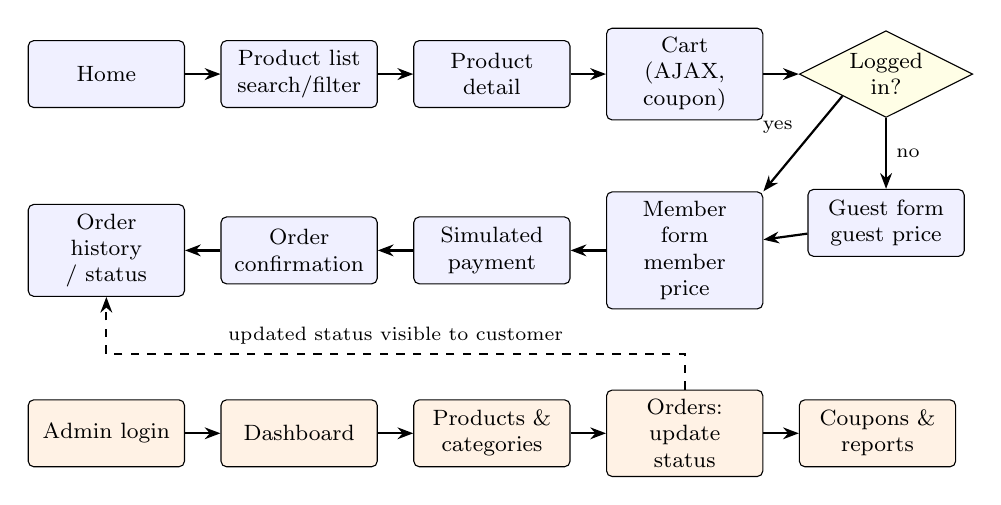
\begin{tikzpicture}[
  node distance=0.45cm and 0.45cm,
  box/.style={draw,rounded corners=2pt,align=center,font=\footnotesize,
              minimum height=0.85cm,text width=1.75cm,fill=blue!6},
  adm/.style={box,fill=orange!10},
  dec/.style={draw,diamond,aspect=2,align=center,font=\footnotesize,inner sep=1pt,fill=yellow!10},
  arr/.style={-{Stealth[length=2mm]},thick}
]
% customer flow
\node[box] (home) {Home};
\node[box,right=of home] (list) {Product list\\search/filter};
\node[box,right=of list] (detail) {Product detail};
\node[box,right=of detail] (cart) {Cart\\(AJAX, coupon)};
\node[dec,right=of cart] (logged) {Logged\\in?};
\node[box,below=0.9cm of logged] (guest) {Guest form\\guest price};
\node[box,below=0.9cm of cart] (member) {Member form\\member price};
\node[box,left=of member] (pay) {Simulated payment};
\node[box,left=of pay] (confirm) {Order\\confirmation};
\node[box,left=of confirm] (status) {Order history / status};

\draw[arr] (home) -- (list);
\draw[arr] (list) -- (detail);
\draw[arr] (detail) -- (cart);
\draw[arr] (cart) -- (logged);
\draw[arr] (logged) -- node[right,font=\scriptsize]{no} (guest);
\draw[arr] (logged.south west) -- node[above left,font=\scriptsize]{yes} (member.north east);
\draw[arr] (guest) -- (member);
\draw[arr] (member) -- (pay);
\draw[arr] (pay) -- (confirm);
\draw[arr] (confirm) -- (status);

% admin flow
\node[adm,below=1.3cm of status] (alogin) {Admin login};
\node[adm,right=of alogin] (dash) {Dashboard};
\node[adm,right=of dash] (prod) {Products \&\\categories};
\node[adm,right=of prod] (ord) {Orders: update status};
\node[adm,right=of ord] (rep) {Coupons \&\\reports};
\draw[arr] (alogin) -- (dash);
\draw[arr] (dash) -- (prod);
\draw[arr] (prod) -- (ord);
\draw[arr] (ord) -- (rep);
\draw[arr,dashed] (ord.north) -- ++(0,0.45) -| node[pos=0.25,above,font=\scriptsize]{updated status visible to customer} (status.south);
\end{tikzpicture}

{\small Figure 1. Main customer flow (blue; the guest form path is shown for readability) and administrator flow (orange).}
\end{center}

\begin{center}
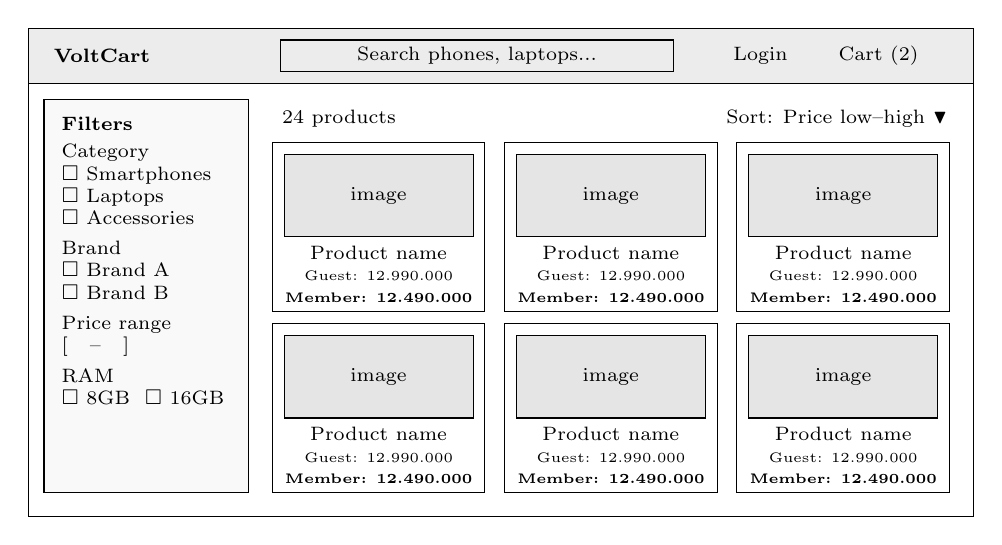
\begin{tikzpicture}[font=\scriptsize]
  \draw (0,0) rectangle (12,6.2);
  % header
  \draw[fill=gray!15] (0,5.5) rectangle (12,6.2);
  \node[anchor=west] at (0.2,5.85) {\textbf{\ProjectName}};
  \draw (3.2,5.65) rectangle (8.2,6.05); \node at (5.7,5.85) {Search phones, laptops...};
  \node at (9.3,5.85) {Login};
  \node at (10.8,5.85) {Cart (2)};
  % sidebar filters
  \draw[fill=gray!5] (0.2,0.3) rectangle (2.8,5.3);
  \node[anchor=north west,align=left] at (0.3,5.2)
       {\textbf{Filters}\\[2pt] Category\\ $\square$ Smartphones\\ $\square$ Laptops\\
        $\square$ Accessories\\[3pt] Brand\\ $\square$ Brand A\\ $\square$ Brand B\\[3pt]
        Price range\\ {[}\quad--\quad{]}\\[3pt] RAM\\ $\square$ 8GB \ $\square$ 16GB};
  % sort bar
  \node[anchor=west] at (3.1,5.05) {24 products};
  \node[anchor=east] at (11.8,5.05) {Sort: Price low--high $\blacktriangledown$};
  % product grid
  \foreach \x in {0,1,2}{
    \foreach \y in {0,1}{
      \begin{scope}[shift={(3.1+\x*2.95,0.3+\y*2.3)}]
        \draw (0,0) rectangle (2.7,2.15);
        \draw[fill=gray!20] (0.15,0.95) rectangle (2.55,2.0);
        \node at (1.35,1.47) {image};
        \node at (1.35,0.75) {Product name};
        \node[font=\tiny] at (1.35,0.45) {Guest: 12.990.000};
        \node[font=\tiny] at (1.35,0.18) {\textbf{Member: 12.490.000}};
      \end{scope}}}
\end{tikzpicture}

{\small Figure 2. Low-fidelity wireframe of the product listing page (desktop). On mobile the
filter sidebar collapses into a ``Filters'' button and the grid becomes one or two columns.}
\end{center}

\section{Proposed Technology Stack}

\begin{tabularx}{\linewidth}{|l|Y|}
\hline
\rowcolor{gray!15} \textbf{Layer} & \textbf{Choice and reason} \\ \hline \endhead
Backend   & PHP 8.2 + Laravel 11 (recommended by the course; built-in auth, validation, migrations, seeders). \\ \hline
Frontend  & Hand-written HTML5 + CSS3 without a CSS framework: Flexbox/Grid for layout, CSS variables
            (\texttt{:root}) for consistent colors and fonts, media queries for responsiveness. Pages are placed
            in Laravel Blade templates to display data from the database. Vanilla JavaScript (\texttt{fetch})
            for AJAX (cart quantity, coupon, search suggestions). \\ \hline
Database  & MySQL 8 (via XAMPP/Laragon locally); schema managed by Laravel migrations. \\ \hline
Charts    & Chart.js for the dashboard sales chart (optional for core). \\ \hline
Tools     & Git + GitHub (feature branches, pull requests), Figma or draw.io for wireframes, VS Code. \\ \hline
\end{tabularx}

\section{Development Plan (8 Weeks)}

\begin{tabularx}{\linewidth}{|l|Y|}
\hline
\rowcolor{gray!15} \textbf{Week} & \textbf{Main tasks} \\ \hline \endhead
1--2 & Form team, choose product category, research reference websites, personas, wireframes,
       create Git repository with the mandatory folder structure. \\ \hline
3 (CP1) & Present Checkpoint 01; finalize database design (ERD); Laravel project setup; shared CSS file
       (colors, fonts, buttons, forms, grid) and base HTML layout (header, footer, navigation). \\ \hline
4    & Migrations and seeders with realistic sample data; authentication; product listing and detail
       from the database; admin product and category CRUD. \\ \hline
5    & Cart with AJAX; guest checkout; member price; basic admin order management. \\ \hline
6 (CP2) & Present working core flow; coupon rule; order status update and customer view;
       responsive fixes; progress note. \\ \hline
7    & Dashboard and sales report; profile and order history; validation messages;
       write and run test cases; start selected advanced features. \\ \hline
8 (CP3) & Feature freeze; bug fixing; complete \texttt{TEST\_CASES.xlsx}, final report, setup
       instructions and demo video; final submission. \\ \hline
\end{tabularx}

\section{Repository and Initial Work}

Repository: \RepoURL. The repository already follows the mandatory structure
(\texttt{CODE/}, \texttt{DATABASE/}, \texttt{DATA/}, \texttt{DOCUMENTATION/}, \texttt{VIDEO/},
\texttt{README.md}). Workflow: \texttt{main} (stable) and \texttt{develop} branches,
one feature branch per task (e.g.\ \texttt{feature/cart-ajax}), merged through pull requests
reviewed by another member. Initial commits: folder structure, README, \texttt{STUDENT\_INFO.md},
wireframes, and this report.

\newpage
% =====================================================================
\part*{\large Part B -- Mini-Research Report}
% =====================================================================

\section{Reference Websites}

We studied three popular electronics retailers in Vietnam that sell both smartphones and laptops:

\begin{enumerate}
  \item \textbf{Thế Giới Di Động} -- \url{https://www.thegioididong.com}:
        nationwide chain with a very large catalog; strong filtering and a detailed
        specification table on every product page.
  \item \textbf{FPT Shop} -- \url{https://fptshop.com.vn}:
        large retailer with a clean product layout, many promotions and a product comparison feature.
  \item \textbf{CellphoneS} -- \url{https://cellphones.com.vn}:
        popular with students; runs a membership program (Smember) with special member prices,
        which is very close to our guest/member pricing requirement.
\end{enumerate}

\section{Target Customers and Personas}

Our target customers are students and young professionals who buy a device for study or work,
have a limited budget, and shop mainly on their phones.

\begin{tabularx}{\linewidth}{|L{2.3cm}|Y|Y|}
\hline
\rowcolor{gray!15}  & \textbf{Persona 1 -- Minh (guest buyer)} & \textbf{Persona 2 -- Lan (member)} \\ \hline \endhead
Profile     & 19, first-year IT student, budget about 15 million VND. &
              27, office worker, buys accessories and upgrades her phone every 2--3 years. \\ \hline
Goal        & Find a laptop with at least 16GB RAM for programming. &
              Get the best price and track her orders easily. \\ \hline
Pain points & Too many models and banners; does not want to create an account for one purchase. &
              Re-entering address every time; unclear final price after promotions. \\ \hline
Needs from us & Simple filters (price, RAM), clear stock status, fast guest checkout. &
              Member price, saved profile and address, order history and status. \\ \hline
\end{tabularx}

\section{Feature Comparison}

% TODO (team): re-check every cell on the live websites and add screenshots in the appendix.
\begin{center}
\begin{tabularx}{\linewidth}{|Y|c|c|c|c|}
\hline
\rowcolor{gray!15} \textbf{Feature} & \textbf{TGDĐ} & \textbf{FPT Shop} & \textbf{CellphoneS} & \textbf{\ProjectName} \\ \hline \endhead
Category menu and featured products        & \yes & \yes & \yes & \yes \\ \hline
Search with suggestions                    & \yes & \yes & \yes & \yes \\ \hline
Filter by brand / price / specifications   & \yes & \yes & \yes & \yes \\ \hline
Sorting by price                           & \yes & \yes & \yes & \yes \\ \hline
Detailed specification table               & \yes & \yes & \yes & \yes \\ \hline
Stock / availability information           & \yes & \yes & \yes & \yes \\ \hline
Guest checkout without account             & \yes & \yes & \yes & \yes \\ \hline
Member price / membership program          & \half & \half & \yes & \yes \\ \hline
Coupon / voucher code                      & \yes & \yes & \yes & \yes (one rule) \\ \hline
Order tracking                             & \yes & \yes & \yes & \yes \\ \hline
Product comparison                         & \yes & \yes & \yes & stretch goal \\ \hline
Installment payment                        & \yes & \yes & \yes & \no \\ \hline
Trade-in program                           & \yes & \yes & \yes & \no \\ \hline
Customer reviews and ratings               & \yes & \yes & \yes & \no \\ \hline
Real online payment gateway                & \yes & \yes & \yes & \no (simulated) \\ \hline
\end{tabularx}

{\small \yes{} available \quad \half{} partial or not prominent \quad \no{} not included}
\end{center}

\section{Selected Features and Reasons}

\textbf{Selected.}
\begin{itemize}
  \item \emph{Filters by brand, price and RAM}: every reference site relies on filters, and
        Persona 1 decides mainly by budget and RAM. We keep only a few filters to stay simple.
  \item \emph{Clear guest and member price on cards, detail, cart and checkout}: inspired by
        CellphoneS member prices; it gives customers a reason to register (Persona 2) and
        satisfies the course requirement.
  \item \emph{Guest checkout}: all three sites allow it; it removes the main pain point of Persona 1.
  \item \emph{AJAX cart and coupon}: instant feedback on quantity and total without reloading the page.
  \item \emph{Order history and status}: needed by members to track deliveries.
\end{itemize}

\textbf{Not selected (and why).}
Installment plans, trade-in, real payment gateways and multiple promotion types are common on
large retailers but require external services and complex rules; they do not fit an 8-week
project. Product variants are replaced by separate products per configuration. Reviews and
product comparison are kept as optional advanced work only after the core flow is stable.

\section{UI/UX Observations}

\begin{itemize}
  \item \textbf{Strengths to adopt:} sticky header with a large search bar; product cards that
        show image, name, key specs and price in a consistent grid; colored stock badges;
        filters that collapse into a button on mobile; a short checkout with an order summary
        always visible.
  \item \textbf{Weaknesses to avoid:} too many promotion banners and pop-ups that push products
        below the fold; several prices on one card (old price, online price, installment price)
        that confuse buyers; very long product pages on mobile.
  \item \textbf{Our design direction:} a clean layout with one accent color, at most two
        prices per product (guest and member, clearly labelled), visible loading, success,
        empty-state and error messages, and a mobile-first responsive grid. All pages are written by the
        team in HTML/CSS (no downloaded template) to keep the design original.
\end{itemize}

\textbf{Reference links:}
\begin{itemize}
  \item Thế Giới Di Động: \url{https://www.thegioididong.com}
  \item FPT Shop: \url{https://fptshop.com.vn}
  \item CellphoneS: \url{https://cellphones.com.vn}
\end{itemize}

\end{document}
